\documentclass[18pt, a0paper, landscape]{tikzposter}
\usepackage[english]{babel}
\usepackage[utf8]{inputenc}
\usepackage{float}
\usepackage[T1]{fontenc}
\usepackage{amsmath}
\usepackage{graphicx}
\graphicspath{{/home/istvan/work/insar/images/}}
\usepackage{siunitx}
\usepackage{caption}
\usepackage{hyperref}
\usepackage{multicol}
\usetikzlibrary{positioning}

\DeclareGraphicsExtensions{.png,.jpg,.jpeg}
\DeclareSIUnit\year{yr}

\title{\parbox{\linewidth}{\centering Attempts to investigate the dynamic
surface changes in the Carpathian bend area using archive ascending and
descending ENVISAT images processed by persistent scatterers interferometry}}
\author{István Bozsó, Eszter Szűcs, László Bányai, Viktor Wesztergom}
\institute{MTA CSFK GGI, Hungary}


\makeatletter
\newcommand\insertlogoi[2][]{\def\@insertlogoi{\includegraphics[#1]{#2}}}
\newcommand\insertlogoii[2][]{\def\@insertlogoii{\includegraphics[#1]{#2}}}
\newlength\LogoSep
\setlength\LogoSep{0pt}

\insertlogoi[height=10cm]{ggi_logo.png}
\insertlogoii[height=5.5cm]{esa_logo.eps}

\renewcommand\maketitle[1][]{  % #1 keys
    \normalsize
    \setkeys{title}{#1}
    % Title dummy to get title height
    \node[transparent,inner sep=\TP@titleinnersep, line width=\TP@titlelinewidth, anchor=north, minimum width=\TP@visibletextwidth-2\TP@titleinnersep]
        (TP@title) at ($(0, 0.5\textheight-\TP@titletotopverticalspace)$) {\parbox{\TP@titlewidth-2\TP@titleinnersep}{\TP@maketitle}};
    \draw let \p1 = ($(TP@title.north)-(TP@title.south)$) in node {
        \setlength{\TP@titleheight}{\y1}
        \setlength{\titleheight}{\y1}
        \global\TP@titleheight=\TP@titleheight
        \global\titleheight=\titleheight
    };

    % Compute title position
    \setlength{\titleposleft}{-0.5\titlewidth}
    \setlength{\titleposright}{\titleposleft+\titlewidth}
    \setlength{\titlepostop}{0.5\textheight-\TP@titletotopverticalspace}
    \setlength{\titleposbottom}{\titlepostop-\titleheight}

    % Title style (background)
    \TP@titlestyle

    % Title node
    \node[inner sep=\TP@titleinnersep, line width=\TP@titlelinewidth, anchor=north, minimum width=\TP@visibletextwidth-2\TP@titleinnersep]
        at (0,0.5\textheight-\TP@titletotopverticalspace)
        (title)
        {\parbox{\TP@titlewidth-2\TP@titleinnersep}{\TP@maketitle}};

    \node[inner sep=0pt,anchor=west]
      at ([xshift=-\LogoSep]title.west)
      {\@insertlogoi};

    \node[inner sep=0pt,anchor=east]
      at ([xshift=\LogoSep]title.east)
      {\@insertlogoii};

    % Settings for blocks
    \normalsize
    \setlength{\TP@blocktop}{\titleposbottom-\TP@titletoblockverticalspace}
}

\makeatother

\tikzposterlatexaffectionproofoff


\begin{document}

\maketitle[width=80cm, roundedcorners=0.5, linewidth=5pt]

\block[roundedcorners=0.5, linewidth=5pt]{Abstract}
{
    Acquired during the ESA scientific project proposal (30142) we have 23
    ascending and 32 descending ENVISAT raw images of the investigated area.
    For the data processing the StaMPS persistent scatterers (Hooper et al.,
    2012) interferometry (PSI) software packages (developed by Andy Hooper) is
    available. This software can estimate the average velocities of persistent
    scatterers (PS) in the line of sight (LOS) directions. Although the LOS
    velocities in ascending (ASC) or descending (DES) directions can
    contribute to the interpretation of the observed processes, the
    combination of ASC and DES velocities can be applied to estimate the
    vertical and east-west components of the velocities, which may be
    distorted by the unknown north-south velocity components. For this
    combination we have to look for close ASC and DES PSs, and determine
    whether they are available in large number. We have developed a program
    package, which selects the close PSs. From the chosen groups of ASC and
    DES PSs, dominant points (DP) are interpolated, where the nearly vertical
    and east-west components are also estimated. We have investigated the
    effects of unknown north-south velocity components. The first attempts of
    combined data processing are also shown and the experienced limitations of
    the environmental effect are summarized.
}


\begin{columns}

    \column{0.25}
    \block[roundedcorners=0.5, linewidth=5pt]{Introduction}
    {
        \begin{center}
            {\Large \color{blue} \underline{Theory}}
        \end{center}

        \vspace{12pt}

        \textbf{Phase difference} terms in a single interferogram (IFG)
        (Hooper et al. 2012):

        \[
            \Delta\Phi = \Phi_{\text{def}} + \Delta\Phi_{\text{DEM}} +
            \Delta\Phi_{\text{atmo}} + \Delta\Phi_{\text{orb}} +
            \Phi_{\text{noise}}
        \]

        \begin{itemize}
            \item $\Phi_{\text{def}}$ - deformation signal
            \item $\Delta\Phi_{\text{DEM}}$ - DEM error phase term
            \item $\Delta\Phi_{\text{atmo}}$ - atmospheric phase term
            \item $\Delta\Phi_{\text{orb}}$ - satellite orbit error phase
            term
            \item $\Phi_{\text{noise}}$ - other noise and error phase
            terms
        \end{itemize}

        \textbf{The task}: estimation of $\Phi_{\text{def}}$ and phase
        \textit{unwrapping}: integration of phase values in the interval
        of $[0, 2\pi)$ so relative deformations can be determined

        \vspace{15pt}

        \begin{center}
            {\Large \color{blue} \underline{Geological background}}
        \end{center}

        \begin{itemize}
            \item \textbf{Ciomadul volcano} - western side of Carpathians-bend
            area
            \item low-resistivity, low-velocity anomaly under Ciomadul
            $\rightarrow$ PAMS volcano: ``volcano with potentially active
            magma storage'' (Harangi et al. 2014)
            \item near the \textbf{Vrancea zone:} subduction zone accompanied by
            intraplate, sub-crustal earthquakes
        \end{itemize}

        \begin{tikzfigure}[Location of the Ciomadul volcano and the
        low-resistivity anomaly under it. The red triangle denotes the
        volcano. Colorscale indicates $\si{\ohm\meter}$ values on logarithmic
        scale. (Harangi et al., 2014)]
            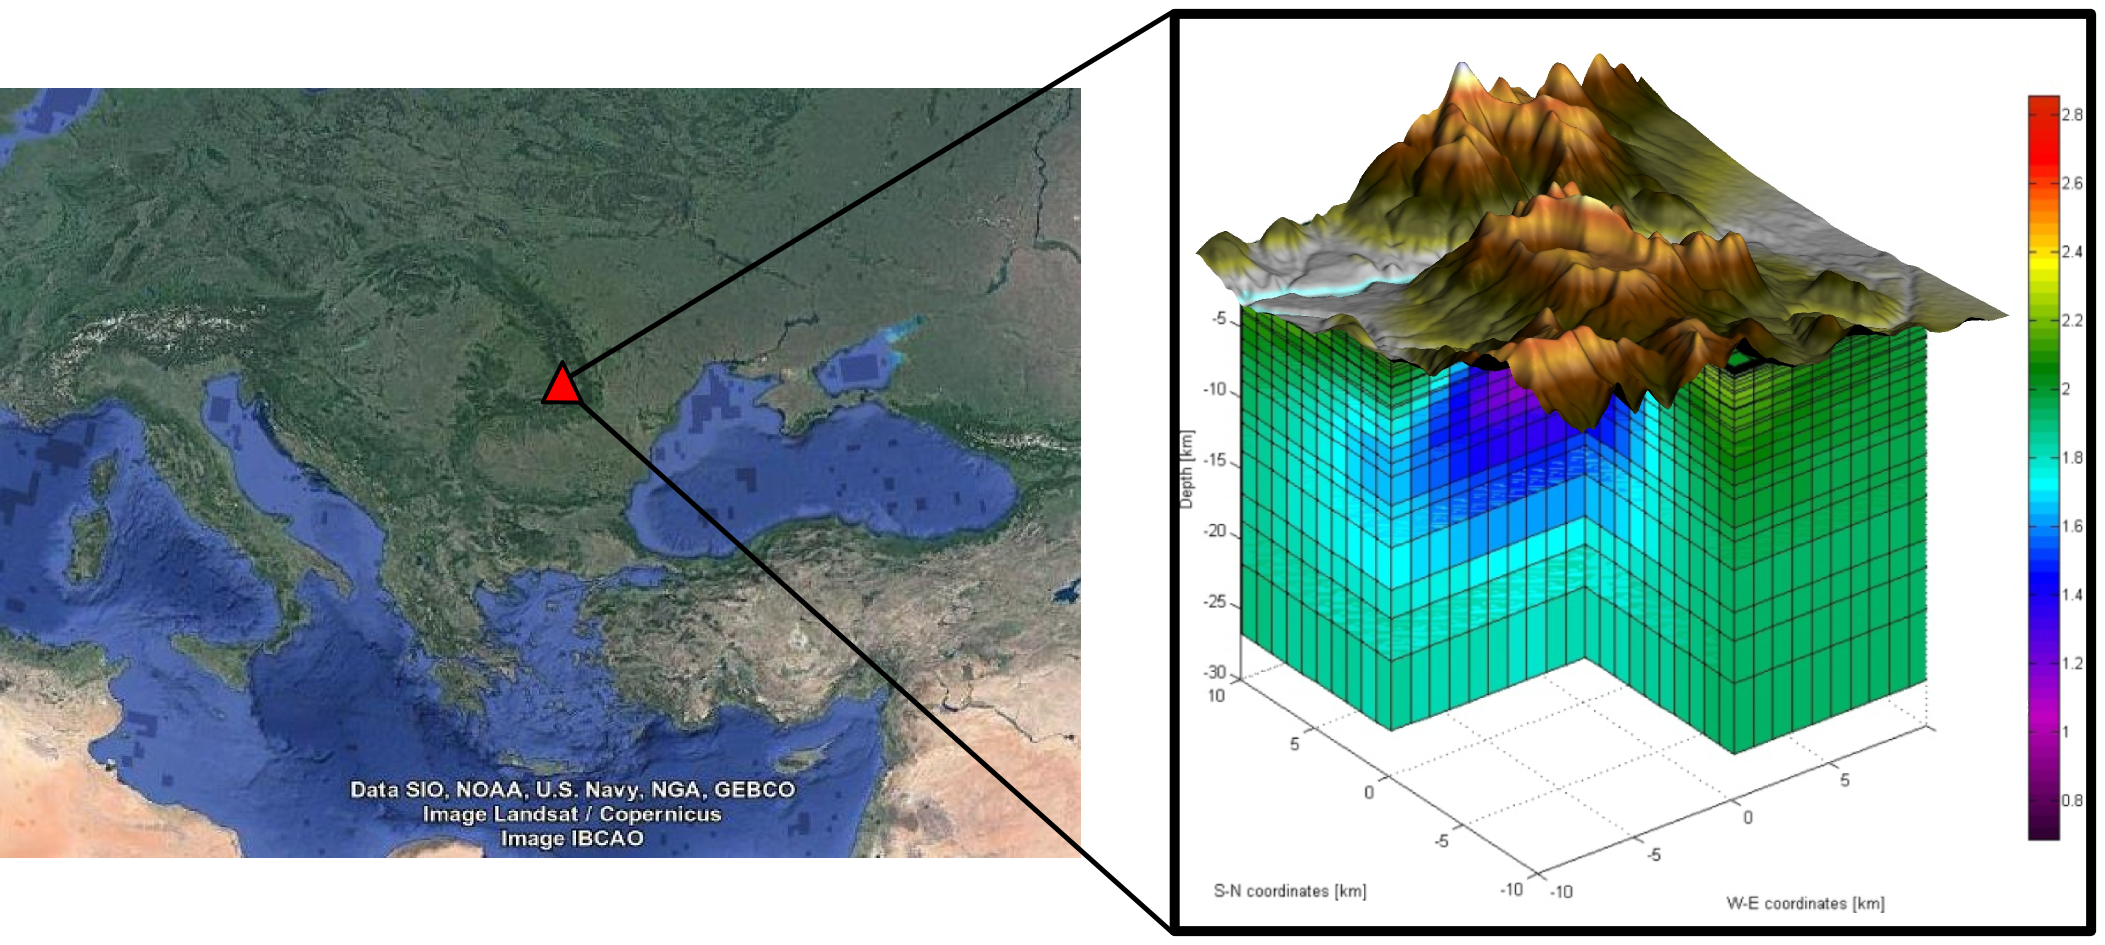
\includegraphics[width=1\linewidth]{google_earth_csomad_harangi.png}
        \end{tikzfigure}

    }

    \column{0.25}

    \block[roundedcorners=0.5, linewidth=5pt]{SBAS processing}
    {
        \begin{itemize}
            \item StaMPS software is capable of both PSI and SBAS
            processing
            \item In our case PSI processing would have yielded very large
            temporal and spatial baselines $\rightarrow$ sporadic clusters of
            coherent pixels mainly around urban aread, IFGs dominated by
            \textbf{incoherence}
            \item We applied the SBAS approach to our dataset
            $\rightarrow$ smaller, temporal and spatial, baselines and more
            coherent IFGs.
        \end{itemize}

        \vspace{25pt}

        \textbf{Setup of the SBAS network:}
        \begin{enumerate}
            \item selection of coherent IFGs
            \item adding less coherent IFGs so coherent ones will be connected
            to the master image and to create redundancy in the network so
            unwrapped phase values could be validated.
        \end{enumerate}

        \begin{center}
            \begin{minipage}[t]{0.49\linewidth}
                \centering
                \begin{tikzfigure}[Ascending SBAS IFG network]
                    \includegraphics[width=1\linewidth]{asc_sb_eng.png}
                \end{tikzfigure}
            \end{minipage}
            \begin{minipage}[t]{0.49\linewidth}
                \centering
                \begin{tikzfigure}[Descending SBAS IFG network]
                    \includegraphics[width=1\linewidth]{des_sb_eng.png}
                \end{tikzfigure}
            \end{minipage}
        \end{center}

        \vspace{25pt}

        \begin{itemize}
            \item many IFGs were discarded, shorter time coverage, low
            redundancy
            \item still some large temporal and spatial baselines are left
            in the network
        \end{itemize}

        \vspace{10pt}

        \begin{flushleft}
            {\Large \color{blue} \underline{Limiting factors}}
        \end{flushleft}

        We could only include 16 IFGs in ASC direction and 24 in DES
        direction, this leftover dataset, however, is still dominated by
        incoherent images. This factor made unwrapping a challange and
        introduced uncertainty to the LOS velocity values, discussed on the
        next column.

    }

    \column{0.25}

    \block[roundedcorners=0.5, linewidth=5pt]{Combined ASC, DES processing}
    {
        \begin{itemize}
            \item Vertical (V) and east-west (EW) velocity components can be
            estimated using the ASC and DES LOS velocities presuming that the
            effects of north-south components can be neglected.
            \item Estimating V and EW components help us understand
            the processes that take place in the area of interest.
            \item The DAISY software developed at the Institute is capable of
            integrating ASC and DES LOS velocities.
            \item The program searches for clusters where both ASC and DES PSs
            can be found in sufficient numbers.
            \item For each cluster DAISY calculates a DP position and
            interpolates vertical and east-west velocities at the DP
            position.
        \end{itemize}

        \vspace{25pt}

        \begin{tikzfigure}[ASC and DES LOS velocities and DP positions.
        Ellipses denote velocities with high standard deviations
        (\numrange{8}{12} $\si{\milli\meter\per\year}$) most likely caused by
        unwrapping errors.]
            \includegraphics[width=1\linewidth]{asc_des_los_dp_std.png}
        \end{tikzfigure}

        \begin{itemize}
            \item LOS velocity standard deviation values can be found
            typically in the range of $1 - \SI{4}{\milli\meter\per\year}$
            \item LOS velocity values are mostly in the range of
            \numrange{-2}{2} $\si{\milli\meter\per\year}$, which means that
            we cannot be certain about the validity of said velocities
        \end{itemize}
    }

    \block[roundedcorners=0.5, linewidth=5pt, bodyinnersep=0.5]{}
    {
        \begingroup
        \renewcommand{\section}[2]{}%
        \tiny
        \begin{flushleft}
            {\small \textbf{References}}
        \end{flushleft}

        \bibliographystyle{apalike}
        \bibliography{../insar}
        \endgroup
    }

    \column{0.25}

    \block[roundedcorners=0.5, linewidth=5pt, bodyinnersep=0.5]{Velocity
    components of the Dominant Points}
    {
        \begin{tikzfigure}[Velocity components of DPs interpolated to a grid
        with linear interpolation. Background: SRTM Digital Elevation Model
        (Jarvis et al, 2008). Colorscale denotes vertical velocity components
        and SRTM heights, arrows show the east-west component. The red
        triangle denotes the volcano.]
            \includegraphics[width=1\linewidth]{grid_dp_vel_red_triang_eng.png}
        \end{tikzfigure}

        \vspace{30pt}

        \innerblock{Conclusions}
        {
            Although the estimated velocities are near to the range of
            estimation error some conclusion can be drawn. However no proper
            natural backscatters could be identified on Ciomadul volcano it is
            rather interesting coincidence that high horizontal movement was
            detected in the wider environment of the volcano. The velocity
            field shows a considerable horizontal eastward movement which
            decreases towards east and tends to downward direction. Upper and
            lower part of the area does not show tendency except a  remarkable
            uplift in the north. The detected movements probably related to
            the subduction ongoing in the Vrancea.
        }
    }


\end{columns}



\end{document}
